\documentclass[10pt, a4paper, twocolumn]{jsarticle}
%
\usepackage{amsmath,amssymb}
\usepackage{bm}
\usepackage{graphicx}
\usepackage{ascmac}
\usepackage{subfigure}
\usepackage{multicol}
\usepackage{setspace}
\usepackage{mediabb}
\usepackage{float}
\usepackage{latexsym}
\usepackage{url}
\usepackage{cite}
\usepackage[top=30truemm,bottom=30truemm,left=25truemm,right=25truemm]{geometry}
%
\setlength{\textwidth}{\fullwidth}
\setlength{\textheight}{39\baselineskip}
\addtolength{\textheight}{\topskip}
\setlength{\voffset}{-0.5in}
\setlength{\headsep}{0.3in}
%
\renewcommand{\baselinestretch}{1.0}
\renewcommand{\figurename}{Fig.}
\renewcommand{\tablename}{Table.}
\renewcommand{\headfont}{\bfseries}


\begin{document}
\twocolumn[
\begin{screen}
\begin{flushleft}
融合情報学輪講資料\hspace{\fill}2014/07/25
\end{flushleft}
\begin{center}
{\Large  Multipath TCPによるデータセンターネットワークの改善  \\
Improving the datacenter network with Multipath TCP}
\end{center}
\begin{flushleft}
工学系研究科 電気系工学専攻 関谷研究室\hspace{\fill}修士課程2年 37-136482 藤居 翔吾
\end{flushleft}
\end{screen}
\vspace{0.5cm}
]
\begin{spacing}{0.7}
\begin{bfseries}
\begin{itshape}
Abstract-
\end{itshape}
As increasing the number of servers in a datacenter, the effective network
topology for utilization of massive computer clusters has been studied.
Recently, using MPTCP for the beneficial use has been tackled this problem.
As another solution, distributed processing system enabled to handle big data.
Today's the technique of distributed processing is that massive workers process data followed by the query from the master nodes.
As the result, a large quantity of short flow is generated in a datacenter network.
MPTCP can achieve the effective consumptions of the resources with multipath,
but a researcher reported MPTCP causes the delay of flow completion for short flows.
In this paper, we verified the utility of the datacenter network with MPTCP, and consider the effects of MPTCP by flow size.

\vspace{0.5cm}
\begin{itshape}
Index-
\end{itshape}
Multipath TCP, Short flow, Flow completion time, FatTree topology, Datacenter
network\end{bfseries}
\end{spacing}
\vspace{0.5cm}
\section{Introduction}
\label{sec:intro}

多様な端末がネットワークに接続できるようになり, 様々な端末から大量かつ多種多様なデータの取得が可能となった.
特にデータ量の増加傾向は顕著で, 18$\sim$24ヶ月単位で総データ容量が2倍になるという予測がされている~\cite{IBM_rep}.
またFacebookでは, 300ペタバイト以上のデータ量を保有しており, 1日あたりに1ペタバイトのデータを解析している~\cite{presto}.
このように近年では, クラウドによるビッグデータの活用が着目され, ウェブ検索, SNSなど,
リアルタイムに近いレスポンスを返すような場面において使われ始めている.
そのようなクラウドサービスには近年要求が高まってきており, Amazonでは100[ms]の遅延により売り上げが1\%下がる,
といった報告~\cite{amazon}があるように, 遅延の影響は深刻な問題となっている.
そのため, 大規模データをより高速に解析することが求められており, データセンターではサーバの運用台数が増加の一途をたどっている.
しかし, 大量の計算機資源から最大限の性能を引き出すためには,
従来の仕組みではデータセンター内トラフィックに対してトラフィックが集中する問題に対応できないため,
計算機資源を有効活用するための研究が盛んに行われている\cite{mapreduce, dryad, fattree, bcube, vl2,
dctcp, improving, detail}.
そのようなスケーラビリティ拡大には, ネットワークトポロジー, アプリケーション, プロトコルに対するアプローチがある.

ネットワークトポロジーを改良するアプローチでは, 従来の単純な階層構造では,
データセンター内で発生するトラフィックに対して帯域が最大限割り当てられない~\cite{fattree}.
そのため, 近年ではそのようなトラフィックに対して帯域を有効利用するトポロジーが提案されている.

大量のデータの処理速度を改良するアプローチでは,
分散処理のためにpartition-aggregate計算モデルが提案されている.
MapReduce~\cite{mapreduce}, Dryad~\cite{dryad}等の分散処理フレームワークは,
この計算モデルに従っており, 今日の大規模クラウドサービスにおいては, 必要不可欠である.

プロトコルを改良するアプローチでは,
従来のTCPを拡張したMultipath TCP
(MPTCP)~\cite{mptcp}をデータセンターネットワークに用いる提案がされている~\cite{fattree,bcube,vl2}.
MPTCPを用いることにより, 複数の経路を同時に利用し, スループットを向上させることが期待されている.

しかし, 分散処理フレームワークを用いることで, フローサイズの小さい大量のQueryが発生し, MPTCPは,
フローサイズの小さいトラフィックに対しては, TCPよりも性能が劣化する問題が報告された~\cite{improving}.
このような背景から, 大規模データセンターネットワークへのMPTCP適用時の問題点を把握するために,
フローサイズの小さいトラフィックに対する性能を検証し,
その原因を分析する.
特に, ns-3シミュレーションを用いたトラフィック解析結果を示し, TCP適用時との比較を行う.

% 本稿では, \ref{sec:related}章でMPTCPによるデータセンターネットワークモデルに関する先行研究を示し,
% \ref{sec:mptcp}章ではMPTCPの詳細を述べる.
% \ref{sec:fattree}章では近年提案されたネットワークトポロジーを紹介し, \ref{sec:traffic_scenario}章では
% データセンター内のトラフィックに関する特性を示す.
% そして, \ref{sec:reproduction}章では報告された問題を検証し,
% \ref{sec:evaluation}章ではデータセンターネットワークでのMPTCPの性能について評価, 考察する.
% 最後に, \ref{sec:conclude}章で本稿での検証結果についてまとめる.

\section{関連研究}
\label{sec:related}
本章では, これまでに報告されている複数経路利用によるフロー完結時間短縮化技術について簡潔に述べ, その優位性や問題点を示す.

2010年にAlizadehらによって, データセンターネットワーク特有のトラフィックパターンに特化して,
パラメータを決定するアルゴリズムが提案された~\cite{dctcp}.
データセンタートラフィックの引き起こす問題点として, キューの生成による遅延, キュー溢れによるパケットロス,
スイッチのバッファに掛かる負荷がある.
これらの問題に対し, キューの蓄積を制御するためのバッファサイズをアルゴリズムから動的に設定することで,
大部分のキューの伝送時間を短縮することを可能にした.
しかし, 大規模計算資源を想定したトポロジーにおける検証がされておらず, また各ネットワークデバイスに細かなチューニングを必要とするため,
大規模データセンターでは運用面での問題がある.

2011年にCostinらによって, MPTCPを用いたデータセンターネットワークモデルが提案された~\cite{improving}.
近年の大規模計算資源を有効活用するために提案されたネットワークトポロジーでは,
高性能なデバイスや特殊な機器を必要とせず, 汎用デバイスのみを用いてホスト同士の通信の際に経路が複数用意されている.
これまでは通信に使わない経路をセカンダリ経路として利用することで, 耐障害性を持たせていたのに対し, 提案されたデータセンターモデルでは,
MPTCPを用い複数経路を同時に利用する事で, 耐障害性を保ちながら, 帯域を最大限利用する事を可能にした.
また, 様々なトポロジーにMPTCPを適用することで, 従来のTCPよりも高いスループットが出せることを示した.
しかし, サイズの小さいフロー($\leq70KB$)のフロー完結時間に着目すると, TCPよりも時間がかかるという問題点があった.

2012年にZarsらによって, 複数レイヤー間でトラフィックを監視し,
しきい値を設定することによるフロー完結時間の短縮化技術を提案した~\cite{detail}.
サイズの異なるフローが混在するネットワークにおいては, サイズが小さいフローがサイズの大きいフローに圧迫され,
伝送遅延が大きくなる問題があったが, この提案では, データリンク層からアプリケーション層までの各層が, 相互にトラフィックを監視する機能をスイッチに実装し,
優先度をつけ, バッファサイズを調整することで, フロー完結時間の悪化を抑えることを可能にした.
しかし, 実験ではClick~\cite{click}を用いて実装を行っており, 現実世界での全てのネットワーク機器の置き換えが必要となるので, 実現は難しい.

以上で述べたことをまとめると, 近年のデータセンターネットワークに対して, 以下のような要求が考えられる.
\begin{itemize}
  \item 大規模計算機を有効活用するトポロジーの利用
  \item 分散処理の際に発生する大量のサイズの小さいフローの送信時間の短縮
  \item 特殊な実装, デバイスを用いず, シームレスな運用の実現
\end{itemize}

\section{データセンターネットワーク}
\label{sec:datacenter}
本章では, データセンターネットワークを構成する技術に関して, その概要を述べる.
\subsection{Multipath TCP}
MPTCPは, 一つの経路でデータ転送するTCPを拡張し, 複数のインタフェース,
あるいは複数のポートを用いてデータ転送をするプロトコルである~\cite{mptcp}.
クライアントが複数のIPアドレスを持っていた場合, 新たにサブフロー\footnote{複数のTCPコネクションの内,
ある一つのコネクションにおけるフロー}のコネクションが確立される.
追加されたサブフローは, クライアントの持つインターフェースが1つの場合, 同じIPアドレスで異なる送受信ポートを用いる.
インターフェースを複数持つ場合には, 異なるIPアドレスの組み合わせで通信を行う.
ルーティングに関しては, 複数の宛先IPアドレス, 送信元アドレスからそれぞれ経路決定される.
このように, アプリケーション層より下のレイヤーのみで複数の経路を使ってデータ転送を行うため,
アプリケーション側がMPTCPでの通信を意識することなくデータ転送ができる.

MPTCPでは, サブフローが, それぞれのシーケンス領域を持ち, 経路状態に合わせて輻輳制御をする~\cite{cong}.
輻輳制御には, TCPと同様にAIMD(additive-increase and
multiplicative-decrease)による輻輳制御がサブフロー単位で行われる.
以下にAIMDアルゴリズムを示す.

\begin{itemize}
\item サブフロー $r$において,
1ACKごとにウィンドウサイズ$\omega_{r}$をmin$(\frac{\alpha}{\omega_{total}},
\frac{1}{\omega_r})$増加させる.
\item サブフロー $r$において, パケットロス時にウィンドウサイズ$\omega_r$を$\frac{\omega_r}{2}$へ減少させる.
\end{itemize}
ここで, $\omega_{total}$は全てのサブフローのウィンドウサイズの総和, $\alpha$は送信速度の増加量を示すパラメータで,
以下のように定義される~\cite{cong}.

\vspace{-2mm}
\begin{eqnarray}
 \alpha = \omega_{total} \times
\frac{\displaystyle \max_{r} \frac{w_r}{RTT^2_r}}{\displaystyle
(\sum_{r}\frac{w_r}{RTT_r})^2}
\label{alpha}
\vspace{-2mm}
\end{eqnarray}

ここで, $RTT_r$はサブフロー$r$でのラウンドトリップ時間を示している.
MPTCPでの輻輳制御には二つの性質ある.
一つは, サブフローのウィンドウサイズは, 全てのウィンドウサイズの大きさに依存するということである.
これにより, 混雑したサブリンクにおいては, ウィンドウサイズが抑えられ, ロードバランスができる.
二つ目は,MPTCPのアルゴリズムによって, TCPでの輻輳制御よりも悪化する事を回避している事である.
しかし, もし複数のサブフローがそれぞれ混雑のないサブリンクを利用する場合, いずれかのコネクションが帯域を占有する可能性がある.

\subsection{FatTreeトポロジーとMPTCPによるデータセンターモデル}
\label{sec:fattree}
この節では, データセンターを構成する要素について述べる.
\subsubsection{トポロジー}
\label{subsec:topology}
従来のデータセンターモデルでは, HostがEdgeスイッチにつながり,
これらのスイッチがAggregationスイッチに集約され,
coreスイッチに接続するといったように, 階層的にトポロジーを形成していた~\cite{fattree}.
このような単純な階層構造を持つトポロジーは, トラフィックの大部分がデータセンター外の通信には有効であった.
しかし, 今日のようなデータセンター内で生じるトラフィックが大半を占める場合, 帯域の割当が適切でなくなる.
このような, データセンター内のトラフィックが主であれば, 階層型のトポロジーはボトルネックを引き起こす可能性がある.
近年の研究~\cite{fattree,bcube,vl2}では, トラフィックがデータセンター内に集中した時の問題を, 物理的なアプローチとして,
トポロジーを工夫する事で解消を試みている.

図\ref{fig:fattree}のように, FatTree~\cite{fattree}では, Coreスイッチを複数用いる事で,
物理パスの最大帯域を供給する.
また, 比較的狭い帯域の経路と汎用的な性能のスイッチを多数用いる.

このようなトポロジーを用いる事で, データセンター内のトラフィックに対し, 帯域を十分に使う事ができる.
しかしこのような密な配置により, 複数の経路が形成され, ルーティングをどのように決定すべきかという問題も生じる事となる~\cite{improving}.
例えば図\ref{fig:fattree}のようなFatTreeトポロジーでは, 4通りの経路が考えられる.
これら複数の経路をリンクエラー時の冗長性を持たせる目的だけでなく, 性能向上に活用することが求められている.
\begin{figure}[h]
    \begin{center}
    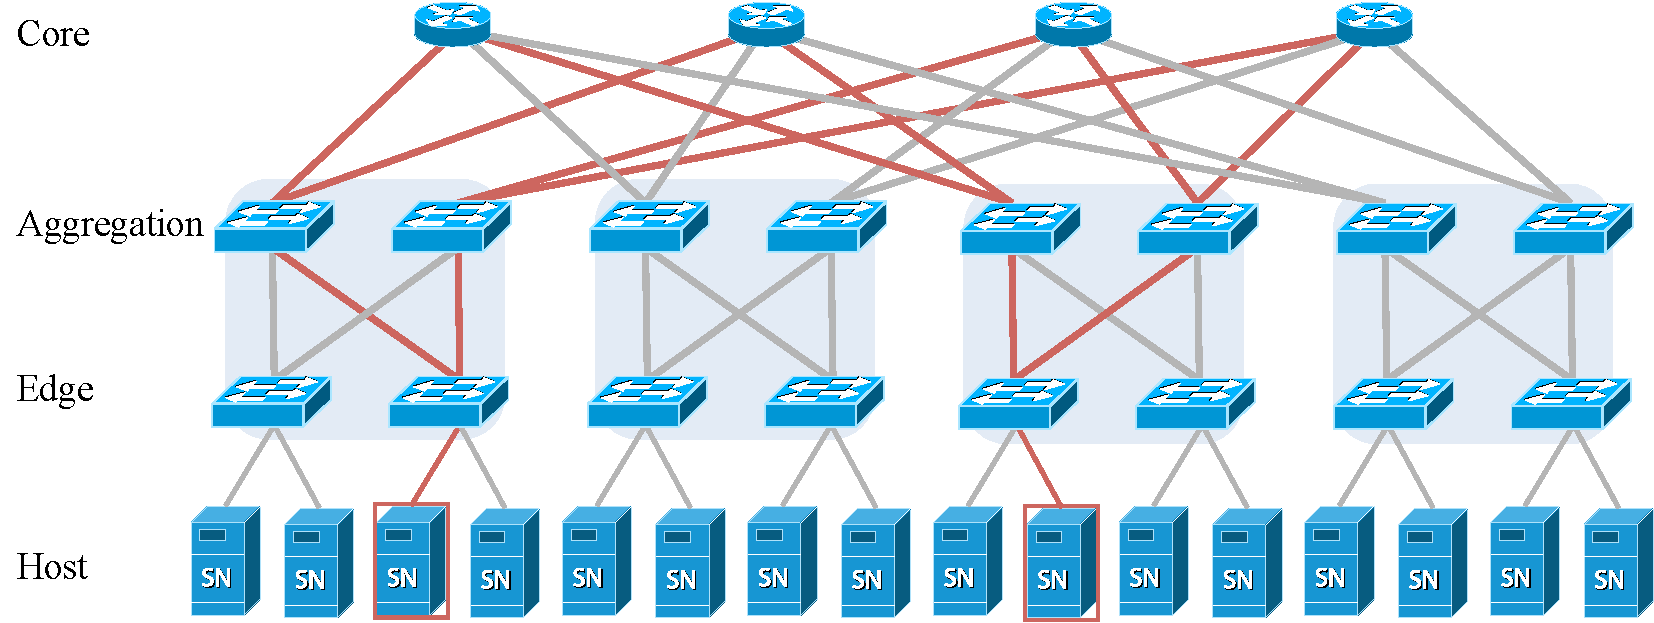
\includegraphics[autoebb, width=210pt]{./img/fattree_topology.pdf}
    \caption{Fattree topology}
    \label{fig:fattree}
    \end{center}
\end{figure}
% \begin{figure}[h]
%     \begin{center}
%     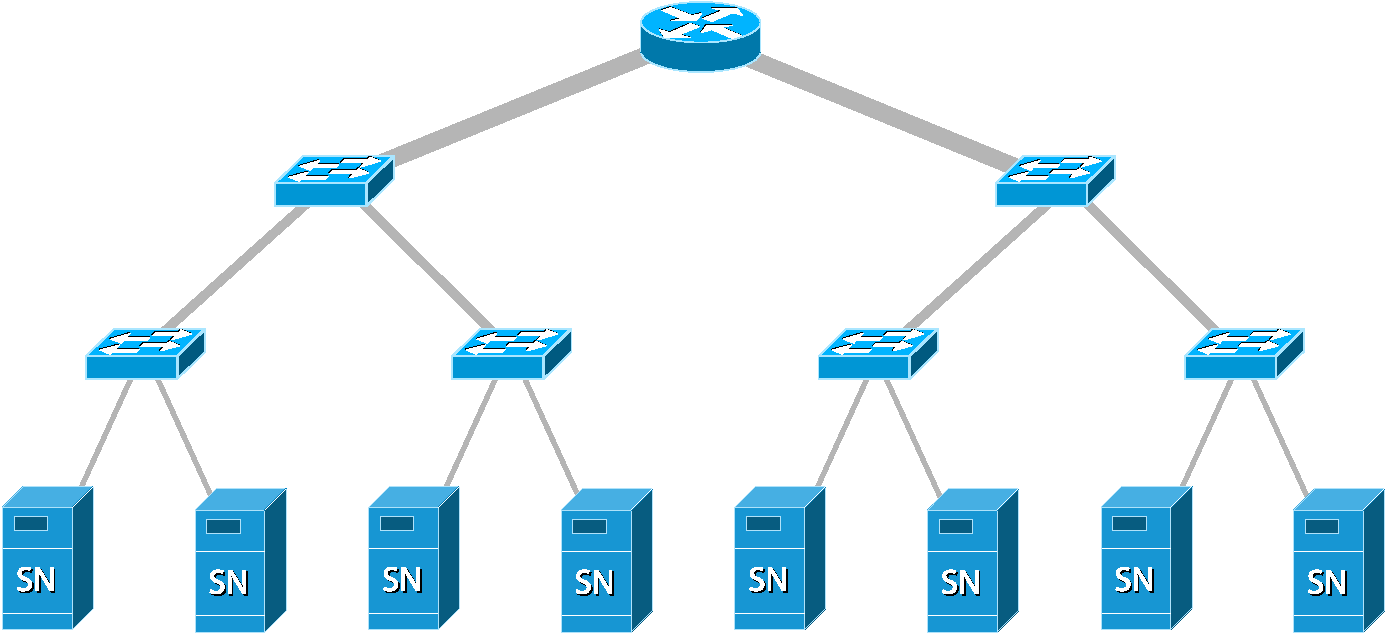
\includegraphics[autoebb, width=180pt]{./img/hierarchy_topology.pdf}
%     \caption{階層型ネットワークトポロジー}
%     \caption{Hierarchical network topology}
%     \label{fig:hierarchical}
%     \end{center}
% \end{figure}

% \begin{figure}[h]
% \begin{minipage}{0.5\hsize}
% \begin{center}
% 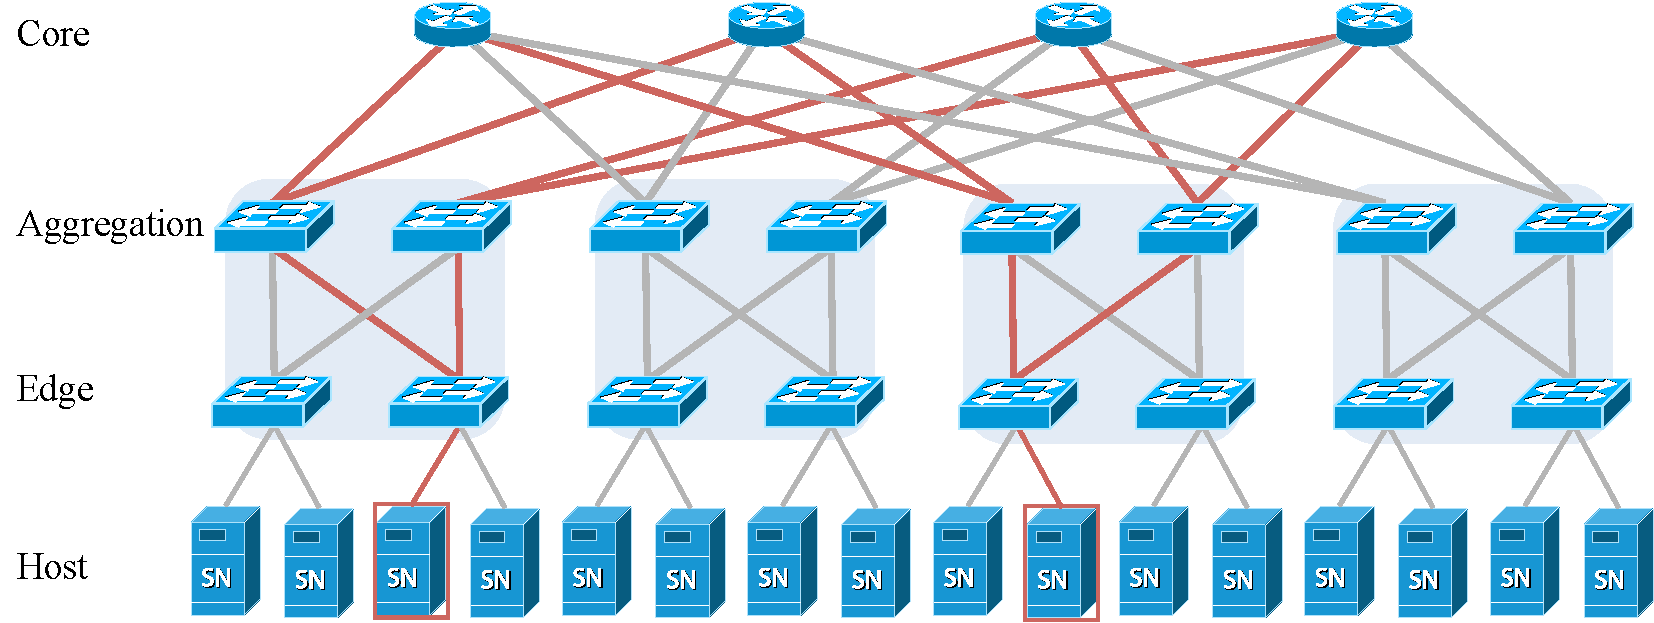
\includegraphics[autoebb, width=110pt]{./img/fattree_topology.pdf}
% \end{center}
% \caption{FatTreeトポロジー}
% \caption{Fattree topology}
% \label{fig:fattree}
% \end{minipage}
% \begin{minipage}{0.5\hsize}
% \begin{center}
% 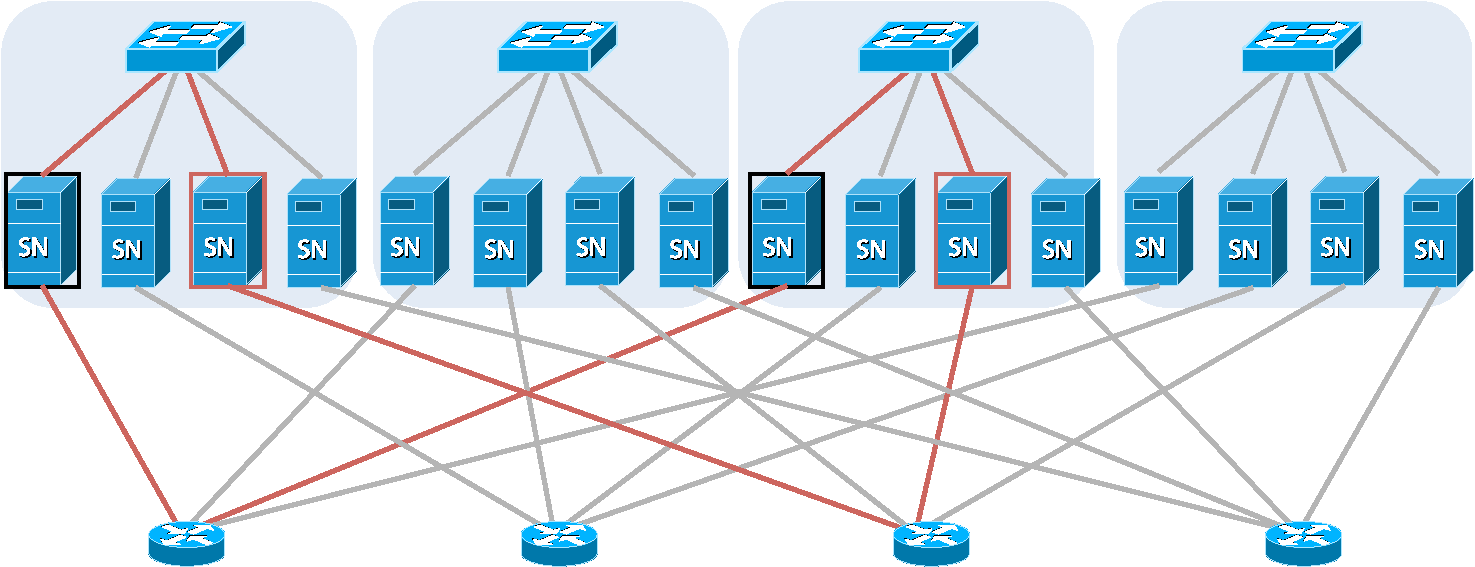
\includegraphics[autoebb, width=110pt]{./img/bcube.pdf}
% \end{center}
% \caption{BCubeトポロジー}
% \caption{BCube topology}
% \label{fig:bcube}
% \end{minipage}
% \end{figure}

\subsection{データセンターにおけるトラフィックシナリオ}
\label{sec:traffic_scenario}
大量の計算機資源を有効活用するためには,
分散処理フレームワークを用い, 一般的に図\ref{fig:part_aggr}に示すようにpartition-aggregate構造をとる.
分散処理フレームワークでは, 多数の処理ノードと分散処理の制御をする管理ノードから構成されており, 管理ノードからQueryが発行され, 分散処理がそれを受け取り,レスポンスを返す.
このとき, トラフィックパターンが  (1){\it Query traffic}, (2){\it Short message
traffic}, (3){\it Backgroung traffic}の3つに分類される~\cite{dctcp}.

{\bf Query traffic. }Query trafficとは, 大規模計算処理を分割して並列処理する際に,
aggregatorノードから処理ノードへ具体的な処理を割り当てるためのトラフィックである.
Query trafficの特徴は, 非常に小さいフローサイズ(2KB$\sim$20KB)で、処理全体の遅延に非常に強く影響を及ぼす事である.
また分散処理システムの構成上, Query trafficはms$\sim \mu$s単位でQueryが生成され,
バースト性を持つと言える~\cite{dctcp}.

{\bf Short message traffic. } Short message trafficとは,
処理ノードの動作を制御するためのトラフィックである.
Short message trafficの特徴は, フローサイズは50KB$\sim$1MBで, Query
trafficと同様に処理全体の遅延に影響を及ぼすという事である.
しかし, Querry trafficほどのフロー数は生成されず, 生成時間間隔も秒単位である.

{\bf Backgroung traffic. }Backgroung trafficは,
各処理ノードへ更新データを送信するトラフィックである.
Backgroung trafficの特徴は,フローサイズが1MB$\sim$50MBと大きいことにある.
さらに, その生成時間間隔は大きい.
また, Backgroung trafficでの更新データは, 処理精度の向上に寄与するが, 処理に必須ではないので,
処理全体の遅延にはつながらない.
また, Alizadehらは, 実際のデータセンターのトラフィックでは, Background trafficが発生する数は少ないが,
全体の通信量の大部分がBackgroung trafficによって占められていると報告しており,
経路全体へ影響を及ぼす可能性があることを示している~\cite{traffic}.

つまり, データセンターネットワークのトラフィックのうち, 分散処理開始時に生成されるQuery trafficが遅延すると,
処理全体に対し遅延を引き起こすので, Query trafficのフロー完結時間は極めて重要なメトリックである.

\begin{figure}[h]
    \begin{center}
    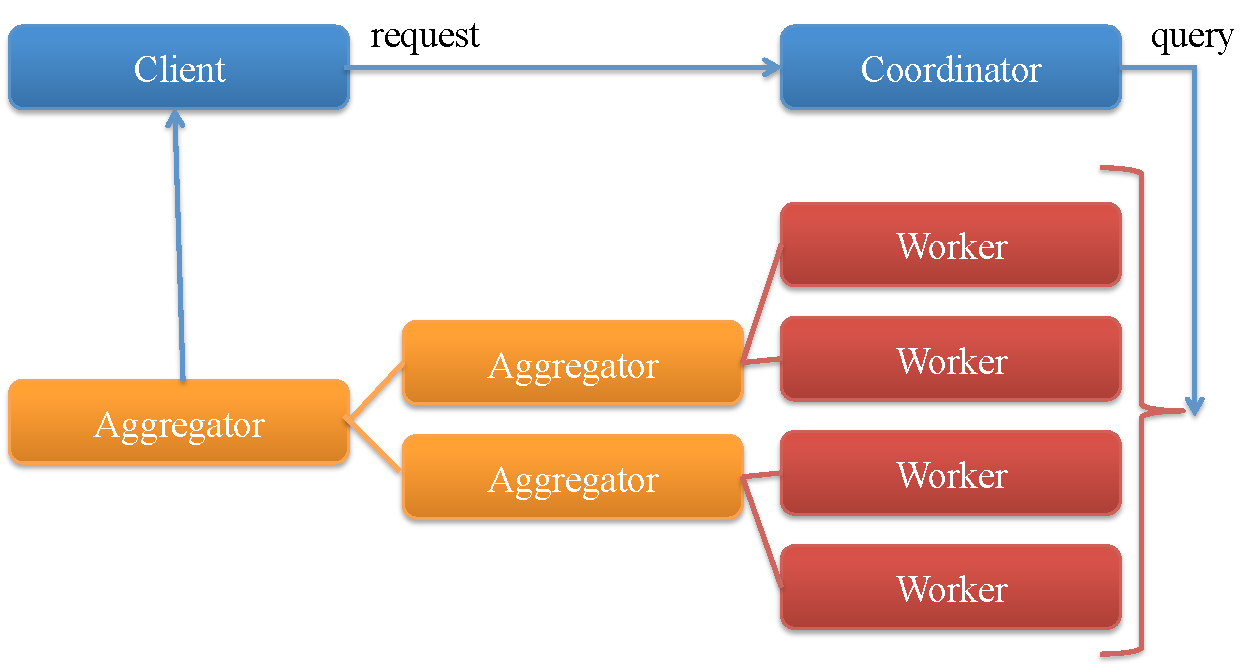
\includegraphics[autoebb, width=210pt]{./img/part_aggr.pdf}
    \caption{Partition-aggregate model on distribution system}
    \label{fig:part_aggr}
    \end{center}
\end{figure}

\section{再現シミュレーション実験}
\label{sec:reproduction}
この章では,
Raiciuらによって示したFatTree-MPTCPネットワークモデルでのフローサイズの小さいトラフィックに対する性能評価シミュレーションを再現し,
解析を行った結果を示す.

\subsection{再現シミュレーション実験環境}
Raiciuらは~\cite{improving}において, 各プロトコルがフローサイズの小さなトラフィックに対して及ぼす影響の評価を行い,
フローサイズの小さいトラフィックに関しては, MPTCPによりフロー完結時間を遅延させることを示した.
そのときのシミュレーション環境は, 以下の通りである.
ネットワークトポロジーには, 4:1にオーバーサブスクリプションされたFatTreeを用いている.
ベンチマークトラフィックについては, ホスト同士の1対1通信を用いている.
全てのホストのうち, 33\%をTCPまたはMPTCPにより継続してデータ転送 (Back-ground traffic)を行う.
残りのhostを使って, TCPによる70Kbyteのデータ転送をを毎200[ms]のポアソン生起させ, 転送完了までにがかかった時間を計測している.

今回の再現実験にはns-3 Direct Code Execution~\cite{ns3}を用い, MPTCPは, Linux
カーネルソースを用いた~\cite{mptcp_linux}.
図\ref{fig:fattree_rep}に, シミュレーションで用いたFatTree(k=2)トポロジーを示す.
このトロポロジーでの物理パスでは, 一つのサブフローが1本の物理パスを占有するように, 設計している.
すなわち, 4つのサブフローを使う場合, ホストの4インターフェースに対しそれぞれ4つIPアドレスが割り当てられる.
また, Host-Edge部分には, IPアドレスの数だけインターフェースを用意し, Aggregation-Edge部分も,
それに従いインターフェースを追加する.
さらにルーティングに関しては, Core1$\sim$Core4に分散するようにルーティングテーブルを設定した.

表\ref{table:testbed}に再現シミュレーション環境に対する各パラメータをまとめる.
\begin{table}[h]
\begin{center}
\footnotesize
\begin{tabular}{c|c}
\hline
Parameter & Value \\ \hline \hline
Nodes & 16 \\
MPTCP & v0.86 \\
Link core-aggr & 400Mbps \\
Link aggr-edge & 200Mbps \\
Link edge-host & 100Mbps \\
RTT & 0.5ms\\
Window size & 100KB \\
\hline
\end{tabular}
\caption{Testbed on network simulation}
\label{table:testbed}
\end{center}
\end{table}

\begin{figure}[h]
    \begin{center}
    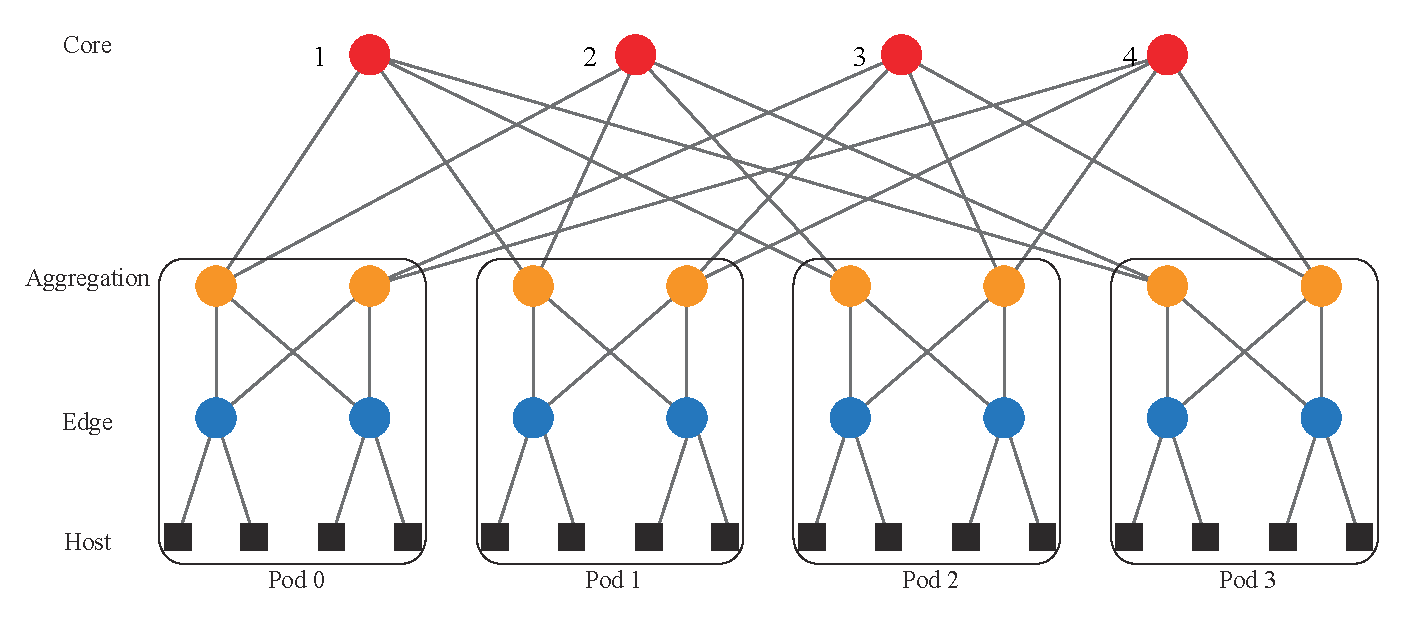
\includegraphics[autoebb, width=210pt]{./img/fattree_rep.pdf}
    \caption{Network topology on reproducing simulation}
    \label{fig:fattree_rep}
    \end{center}
\end{figure}

\subsubsection{設定パラメータに対する有効性の検証}
伝搬遅延についてはRTT(Round Trip Time)として, 0.5[ms]に設定した.
これは, 一般的なデータセンター内のRTTが1[ms]以下であるためである~\cite{rtt}.

ウィンドウサイズについては, 以下の帯域幅遅延積(BDP)の式から, 400Mbpsを最大限利用できるだけの値を設定した.
\vspace{-2mm}
\begin{eqnarray}
BDP[{\rm byte}] = 帯域幅[{\rm bps}] \times RTT \div 8
\label{cong}
\vspace{-2mm}
\end{eqnarray}

各帯域については, 16のノードを使って輻輳を引き起こす現象を再現するために, 実際のデータセンターのような広帯域のネットワークと比べ,
狭い帯域を設定した.

\subsection{再現結果}
図\ref{fig:short_flow_rep}, 表\ref{table:short_flow_rep}に, 上記の実験環境で再現した結果を示す.
再現結果から, フローの様子を完結時間別に4パターンに分類することができることが分かった.
表\ref{table:flow_pattern}にそのフローパターンの定義を示す.

\begin{figure}[h]
    \begin{center}
    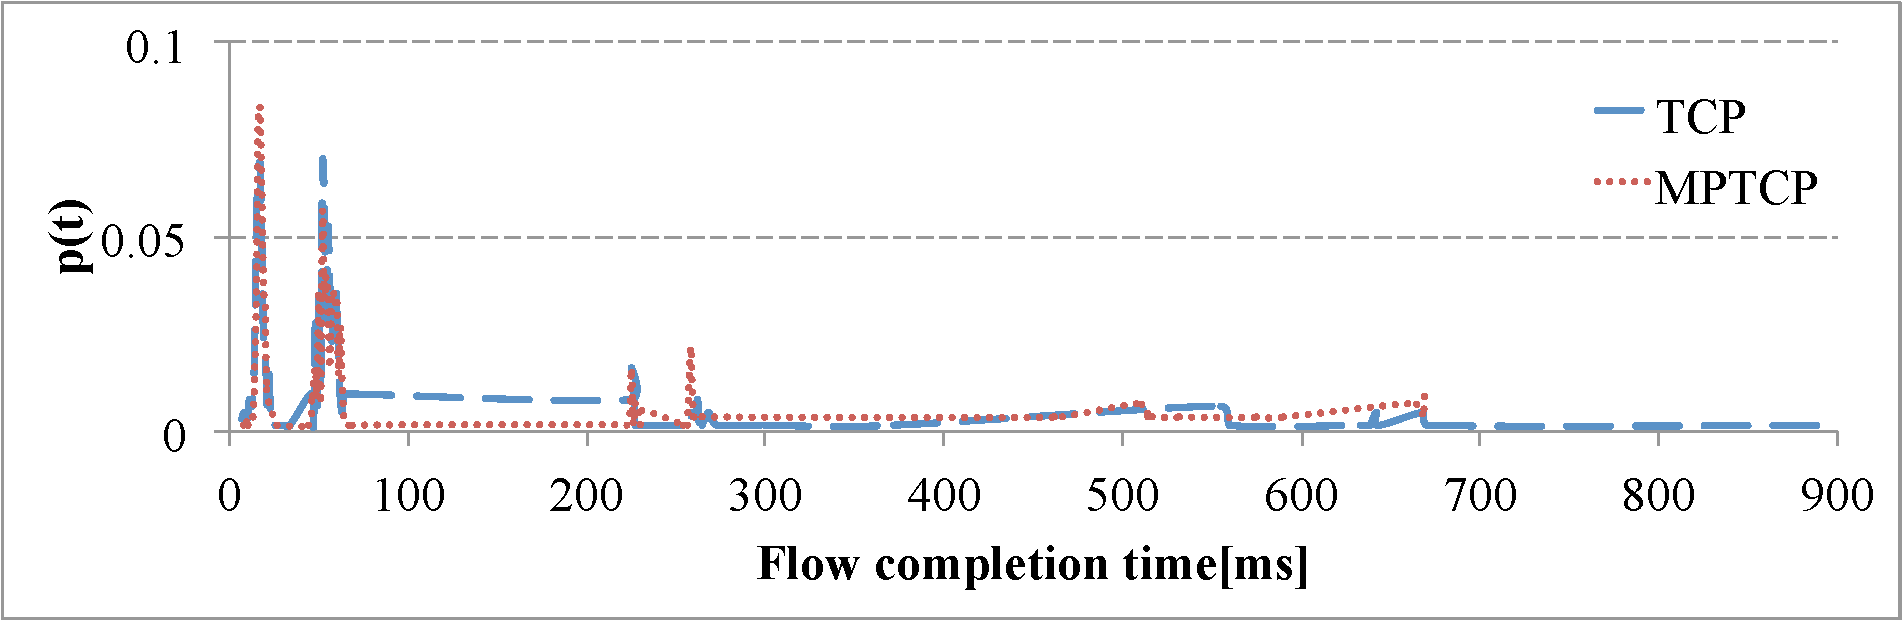
\includegraphics[autoebb, width=210pt]{./img/flow_comp.pdf}
    \caption{The result of the reproduction experiment}
    \label{fig:short_flow_rep}
    \end{center}
\end{figure}

\begin{table}[h]
\begin{center}
\footnotesize
\begin{tabular}{c|p{5em}|p{4em}|p{5em}}
\hline
Protocol & AVG comp time[ms]& Stdev[ms] &
$95^{th}$ percentile[ms]\\
\hline \hline TCP &\hfil 78.4 &\hfil 122.5 &\hfil 266.7\\
MPTCP &\hfil 91 &\hfil 140.6 &\hfil 510.5\\
\hline
\end{tabular}
\caption{Average flow completion time and stdev on reproduction experiment}
\label{table:short_flow_rep}
\end{center}
\end{table}

\begin{table}[h]
\begin{center}
\footnotesize
\begin{tabular}{c|c|c}
\hline
Flow pattern & Comp time[ms] & Packet loss \\ \hline \hline
Full window & $\sim$30 & \\
Intensive flow & $\sim$60 & \\
Delay with loss & 200$\sim$300 & $\surd$\\
Extreme delay & 300$\sim$ & $\surd$\\
\hline
\end{tabular}
\caption{Flow pattern classified by completion time}
\label{table:flow_pattern}
\end{center}
\end{table}

\subsection{考察}
表\ref{table:flow_pattern}に示した各フローパターンについて, それぞれの特性を分析する.

\subsubsection{パケットロスが発生しないフローパターン}
図\ref{fig:full_intensive}にFull windowとIntensive flowのデータ転送の様子を示す.

Full windowでは, TCPコネクション確立後, サーバーがすぐに最大ウィンドウサイズ分だけパケットを送り,
クライアントからのACKが返ってくると, 随時次のパケットを送っていた.
これは, 経路に輻輳がなく, 多くのウィンドウを利用できたということであり, 30[ms]以下でデータ転送を完了した.

一方, Intensive flowでは, サーバーが最大ウィンドウサイズに満たない量のパケットを送り,
クライアントからまとめて送られてくるACKを受け取った後, 集約してパケットを送っていた.
その結果, コネクションの切断時に遅延が起こり60[ms]程度転送時間がかかった.

\subsubsection{パケットロスが生じたフローパターン}
図\ref{fig:delay_loss}にDelay with lossとExtreme delayのデータ転送の様子を示す.
いずれのフローパターンもデータ転送中にパケットロスが発生し, 再送処理, 重複ACK確認応答を行った.
パケットロスが起きた原因は, 短時間にフローサイズの小さいトラフィックが中継ルータを集中したためである.
実際, 200[ms]のポアソン生起のうち, 数10ms単位の短い期間でトラフィックが発生したとき, 中継ルータにおいてパケットロスが生じた.

Delay with lossでは, TCPコネクション確立後に数パケットのデータ転送を行い, パケットロスによるタイムアウトを生じた.
その後, 再送処理を経て, Maximum Segment Size (MSS)である1460[byte]でパケットを伝送した.

一方, Extreme delayでは, TCPコネクション確立直後にパケットロスによるタイムアウトを生じた.
その後も, パケットロスは生じないものの, 400[ms]頃まで伝搬遅延が生じていた.
また, 図\ref{fig:delay_loss}における二つのグラフの傾きは, セグメントサイズ最小値の586[byte]に設定され,
転送速度が上がらなかったことを表している.
これは, 中継するルータにおいてQoE制御による帯域制限が発生したことを示している.
実際, 同時刻に流れていたBackground trafficのスループットには変化がなく, QoE制御のrate controlによりBack-ground
trafficのデータ転送が優先され, ベンチマークトラフィックにはウィンドウサイズが制限されたと考えられる.

\begin{figure}[h]
    \begin{center}
    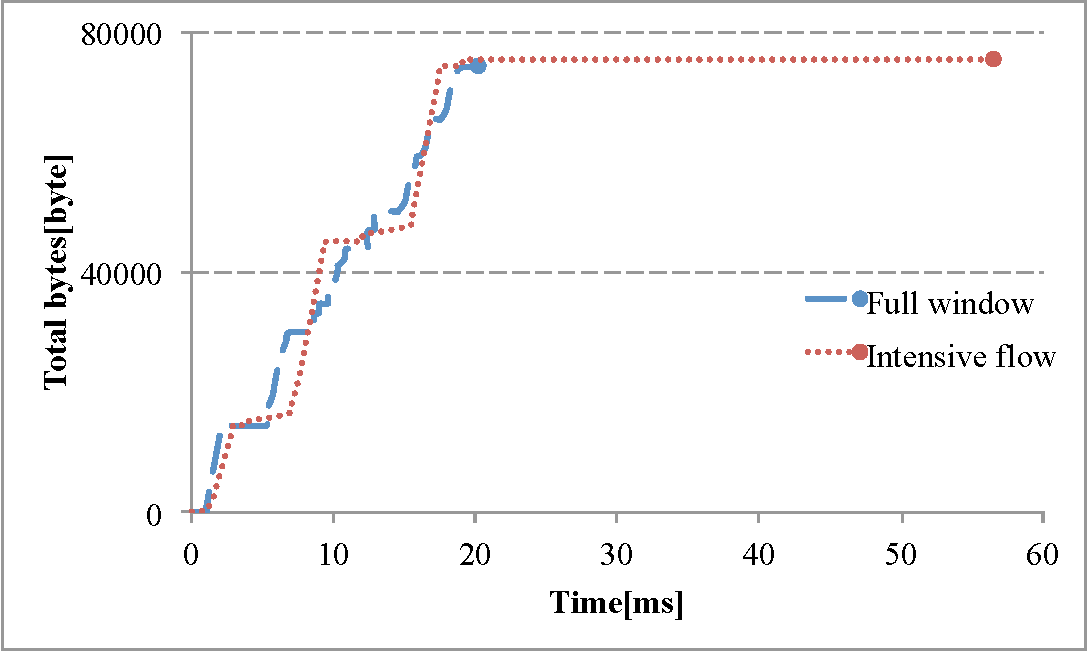
\includegraphics[autoebb, width=210pt]{./img/full_intensive.pdf}
    \caption{Comparison between Full window and Intensive flow}
    \label{fig:full_intensive}
    \end{center}
\end{figure}

\begin{figure}[h]
    \begin{center}
    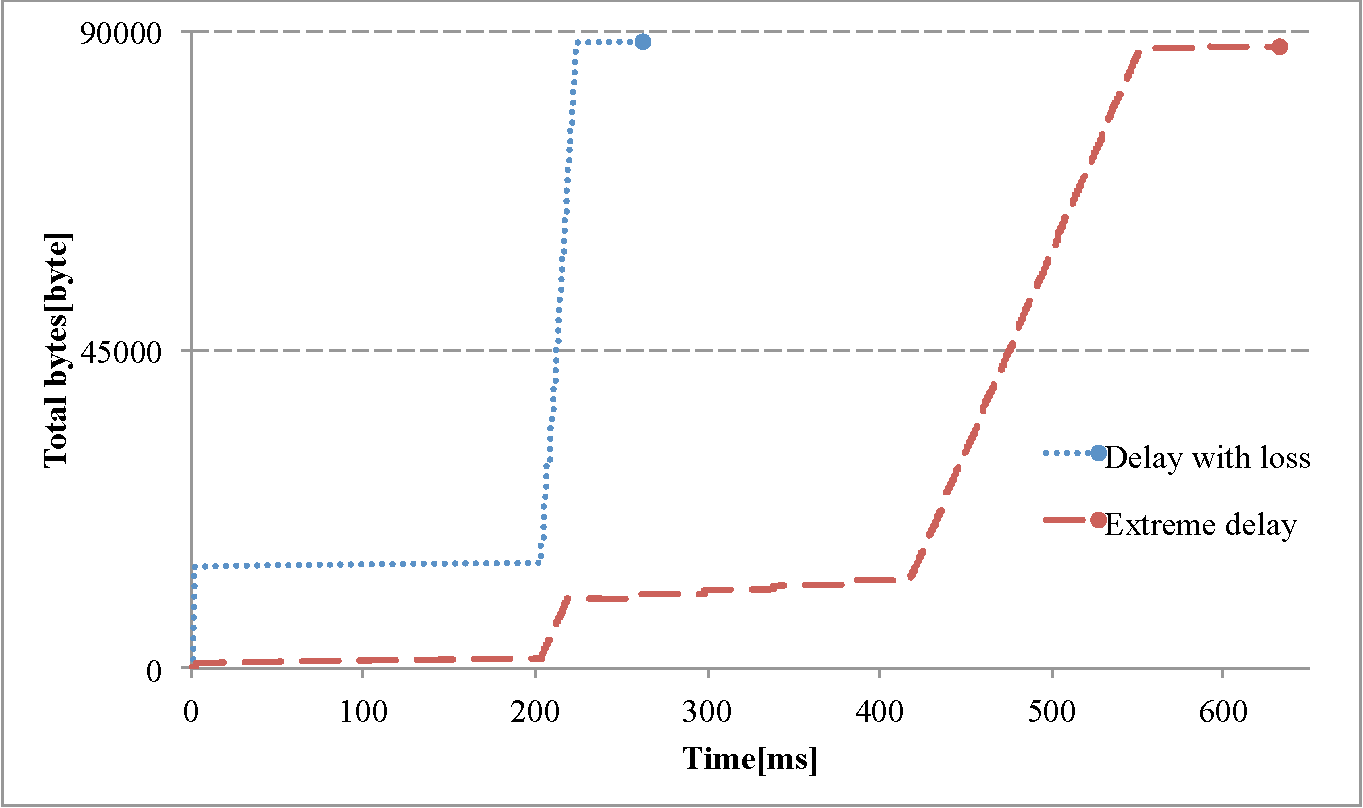
\includegraphics[autoebb, width=210pt]{./img/loss.pdf}
    \caption{Comparison between Delay with loss and Extreme delay}
    \label{fig:delay_loss}
    \end{center}
\end{figure}

\subsubsection{TCP v.s. MPTCP}
今回の再現実験において, TCPとMPTCPでフロー完結時間に差を生じた要因は, パケットロスが発生する割合にある.
図\ref{fig:cdf}に再現実験でのフロー完結時間ごとの累積確率分布を示す.
パケットロスを生じないフローに関しては, 両者に性能差を感じなかったが, この図から, MPTCPを用いた方が,
パケットロスを引き起こし遅延を生じさせる割合が大きいということが分かる.

このようにMPTCPが帯域を大きく占有することにより他のトラフィックを圧迫することは, MPTCPの輻輳制御によるものだと考えられる.
混雑のない経路でデータ転送する場合, MPTCPでは積極的にウィンドウサイズを増やそうとするため, 他のフローに対し遅延を引き起こしたと推測される.


\begin{figure}[h]
    \begin{center}
    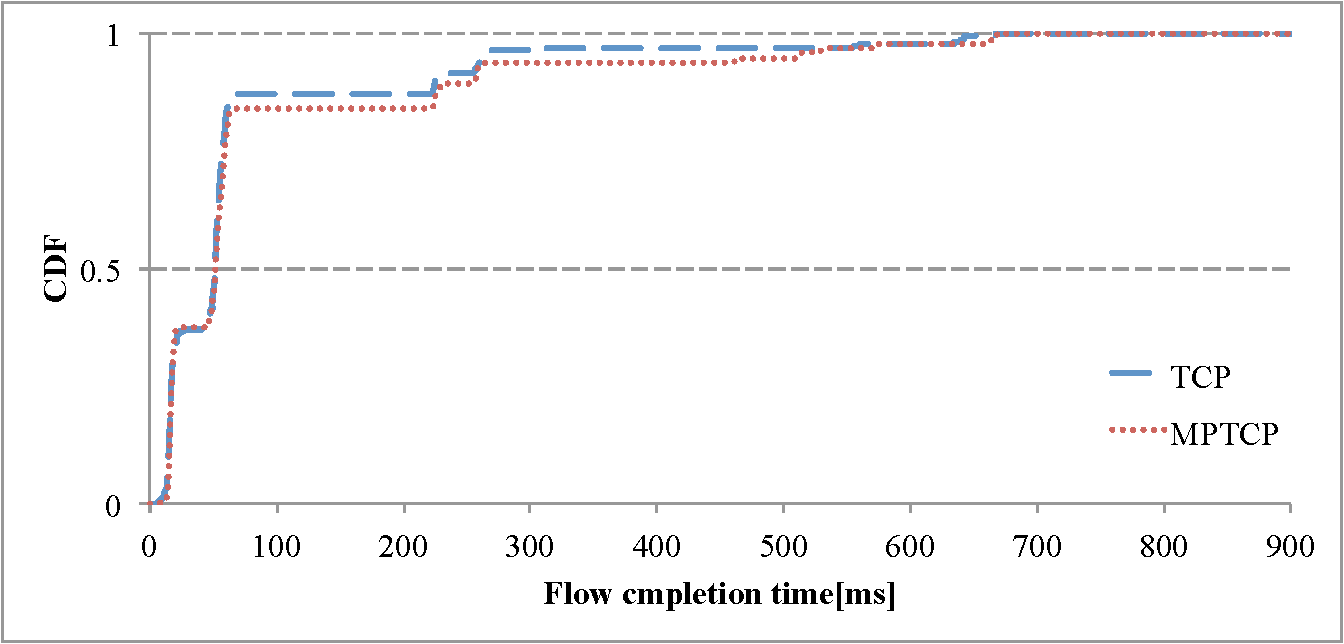
\includegraphics[autoebb, width=210pt]{./img/cdf_rep.pdf}
    \caption{CDF of flow completion time on reproduction experiment}
    \label{fig:cdf}
    \end{center}
\end{figure}

\section{評価実験と考察}
\label{sec:evaluation}
この章では, MPTCPデータセンターネットワークに対して実際のデータセンター環境を想定したシミュレーション実験を行い, その結果について考察する.

\subsection{想定環境}
今回, データセンター上でpartition-aggregateモデルに従う分散処理を想定する.
ネットワークトポロジーについては, 前章のFatTreeトポロジーを用い, 一つのPodが管理ノード群として他Podの12ノードに対し,
処理を指示することを想定する.
またベンチマークトラフィックについては, \ref{sec:traffic_scenario}節で述べた, 2つのトラフィックパターンについて評価・考察を行う.
メトリックとして表\ref{metric}を考える.
\begin{table}[h]
\begin{center}
\footnotesize
\begin{tabular}{c|c}
\hline
Traffic patern & Metric \\ \hline \hline
Query traffic & Comp time[sec] \\
Short message traffic & Comp time[sec] \\
\hline
\end{tabular}
\caption{Metric of each traffic patern}
\label{metric}
\end{center}
\end{table}

\subsection{シミュレーション結果}

\subsubsection{Query traffic}
Query trafficに対する評価として, フローサイズは1[KB]$\sim$16[KB]とした,
12の処理ノードへ平均200[ms]のポアソン生起でトラフィックを発生させ, フロー完結時間を測定した.
また, Query trafficのみ発生させた場合と, 50\%の処理ノードに対し継続的にデータを送信するトラフィックを, Background
trafficとして同時に発生させた場合の2パターンについて評価を行った.
その結果を, 図\ref{fig:pure_query}, \ref{fig:mix_query}に示す.
なお, エラーバーとして99\%信頼区間を採用した.

この結果から, MPTCPはQuery trafficに対し, 直接性能に影響を及ぼさず, Background
Trafficによる影響が性能差を生じさせたことが分かる.
これは, やはりMPTCPがTCPよりも帯域を大きく占有した影響を受けたと考えられる.
\begin{figure}[h]
 \begin{minipage}{0.49\hsize}
  \begin{center}
    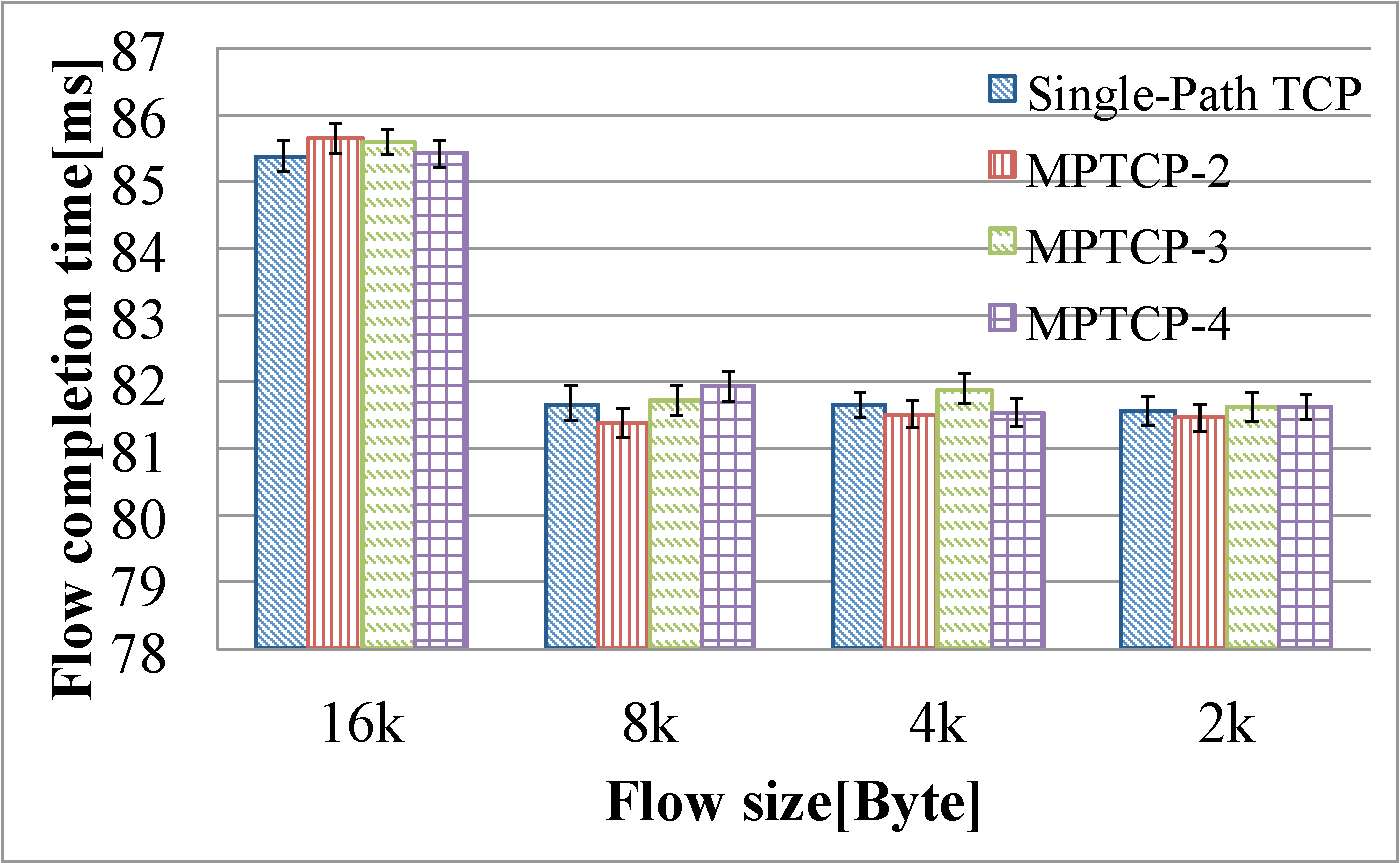
\includegraphics[autoebb, width=95pt]{./img/pure_query.pdf}
    \caption{Flow completion time of Query traffic without Background traffic}
    \label{fig:pure_query}
    \end{center}
 \end{minipage}
 \begin{minipage}{0.49\hsize}
  \begin{center}
    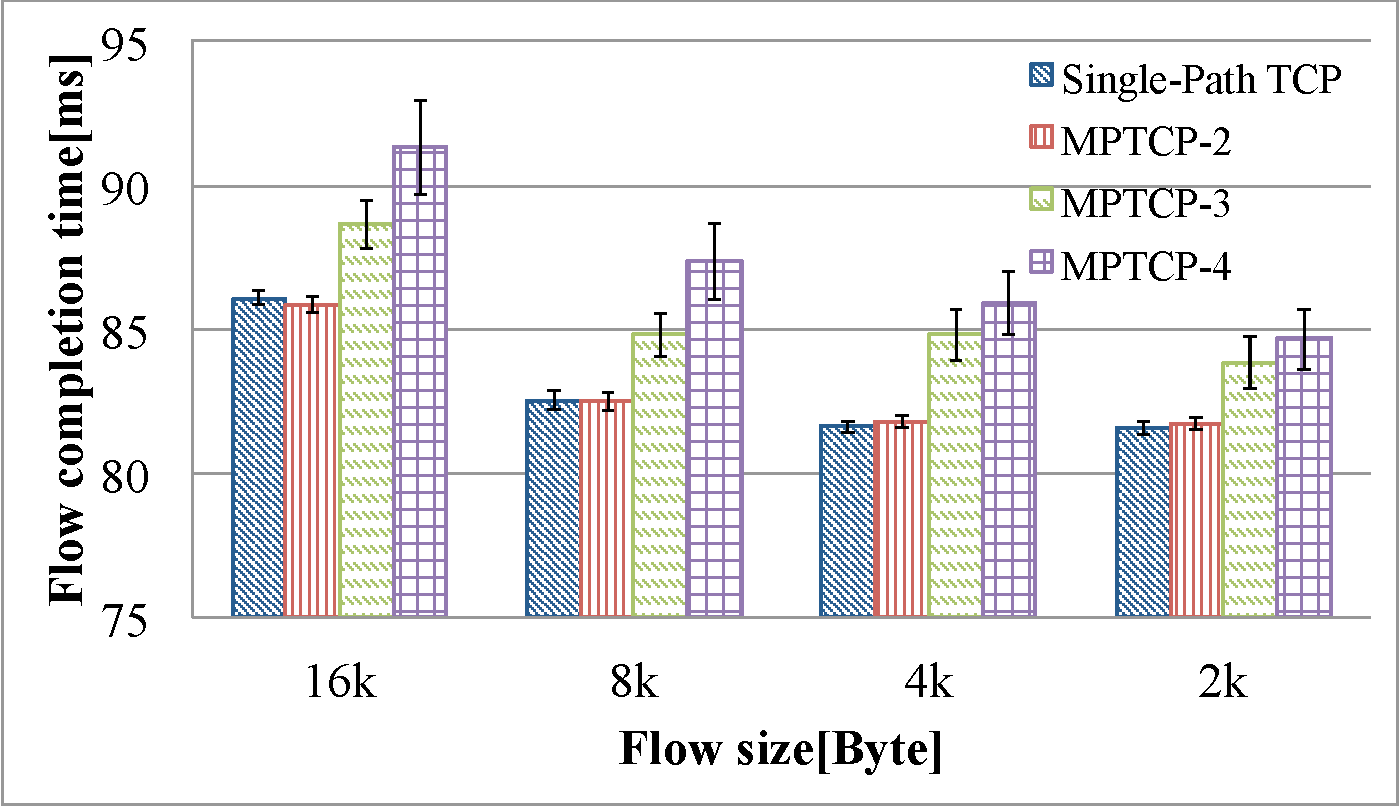
\includegraphics[autoebb, width=95pt]{./img/mix_query.pdf}
    \caption{Flow completion time of Query
    traffic with Background traffic}
    \label{fig:mix_query}
    \end{center}
 \end{minipage}
\end{figure}

\subsubsection{Short message traffic}
Short message trafficに対する評価として, フローサイズは50[KB]$\sim$1[MB]とした.
50\%の処理ノードに対し継続的にデータを送信するトラフィックを, Background trafficとして同時に発生させた状態で,
同時に12の処理ノードへ平均500[ms]のポアソン生起でトラフィックを発生させ, フロー完結時間を測定した.
その結果を, 図\ref{fig:short_query}に示す.

この結果から, MPTCPはShort message trafficに対し, フロー完結時間を短縮させたことが分かる.
これは, 先ほどのQuery trafficよりも大きなサイズのフローを流したので, MPTCPにより複数経路を利用し, TCPよりも短縮したためである.
実際, フローサイズが小さいと, MPTCPとTCP間でフロー完結時間の差が小さくなっている.

\begin{figure}[h]
    \begin{center}
    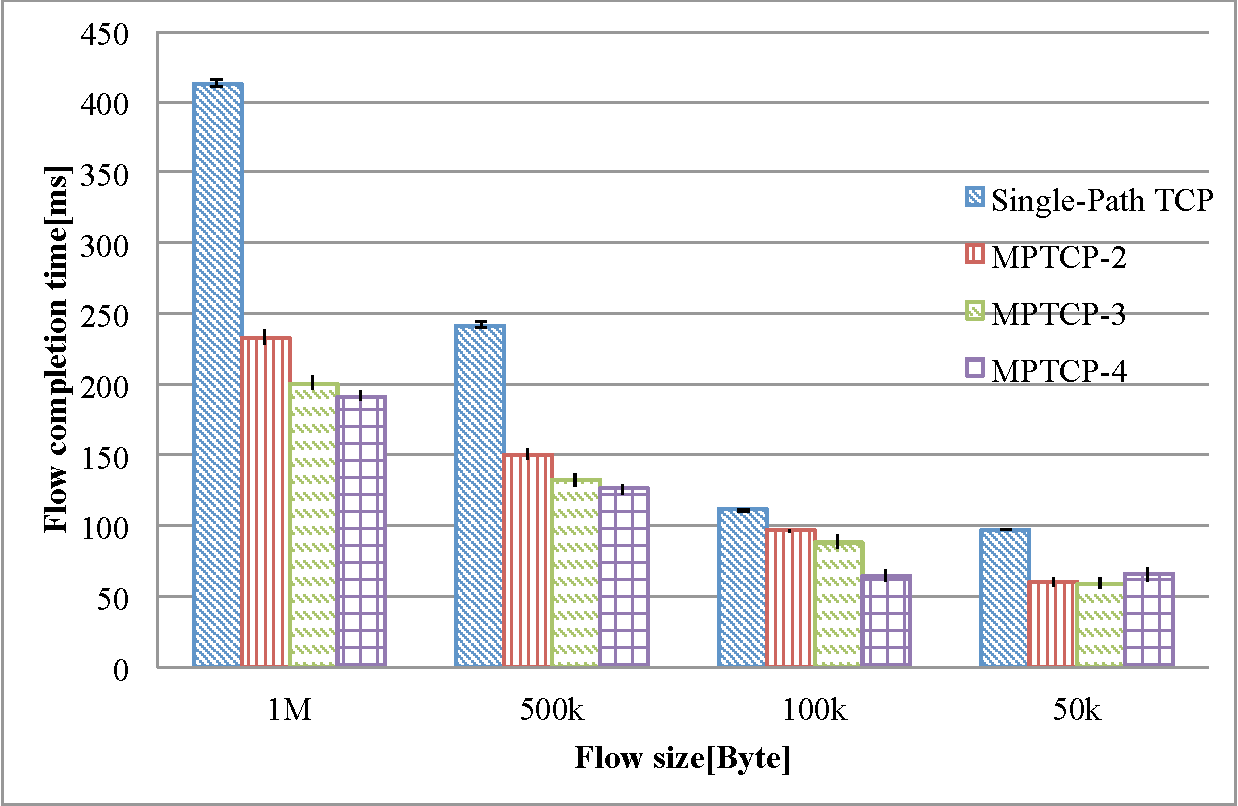
\includegraphics[autoebb, width=210pt]{./img/mix_short.pdf}
    \caption{Flow completion time  of Short message traffic with Background
    traffic}
    \label{fig:short_query}
    \end{center}
\end{figure}


% \subsubsection{Background traffic}
% Background
% trafficに対する評価として全12の処理ノードへ平均500[ms]のポアソン生起でフローサイズ1[KB]$\sim$1[MB]のトラフィックを同時に発生させた状態で,
% 同時に12の処理ノードへ平均500[ms]のポアソン生起でトラフィックを発生させ, 各経路のスループットを計測した.
% その結果を図\ref{fig:background}に示す.
%
% この結果から, MPTCPはBackground trafficに対し, TCPよりも性能向上が見られることが分かる.
% これは, MPTCPのロードバランスと複数経路を使って並行的にデータを送信したことによるものである.
%
% \begin{figure}[h]
%     \begin{center}
%     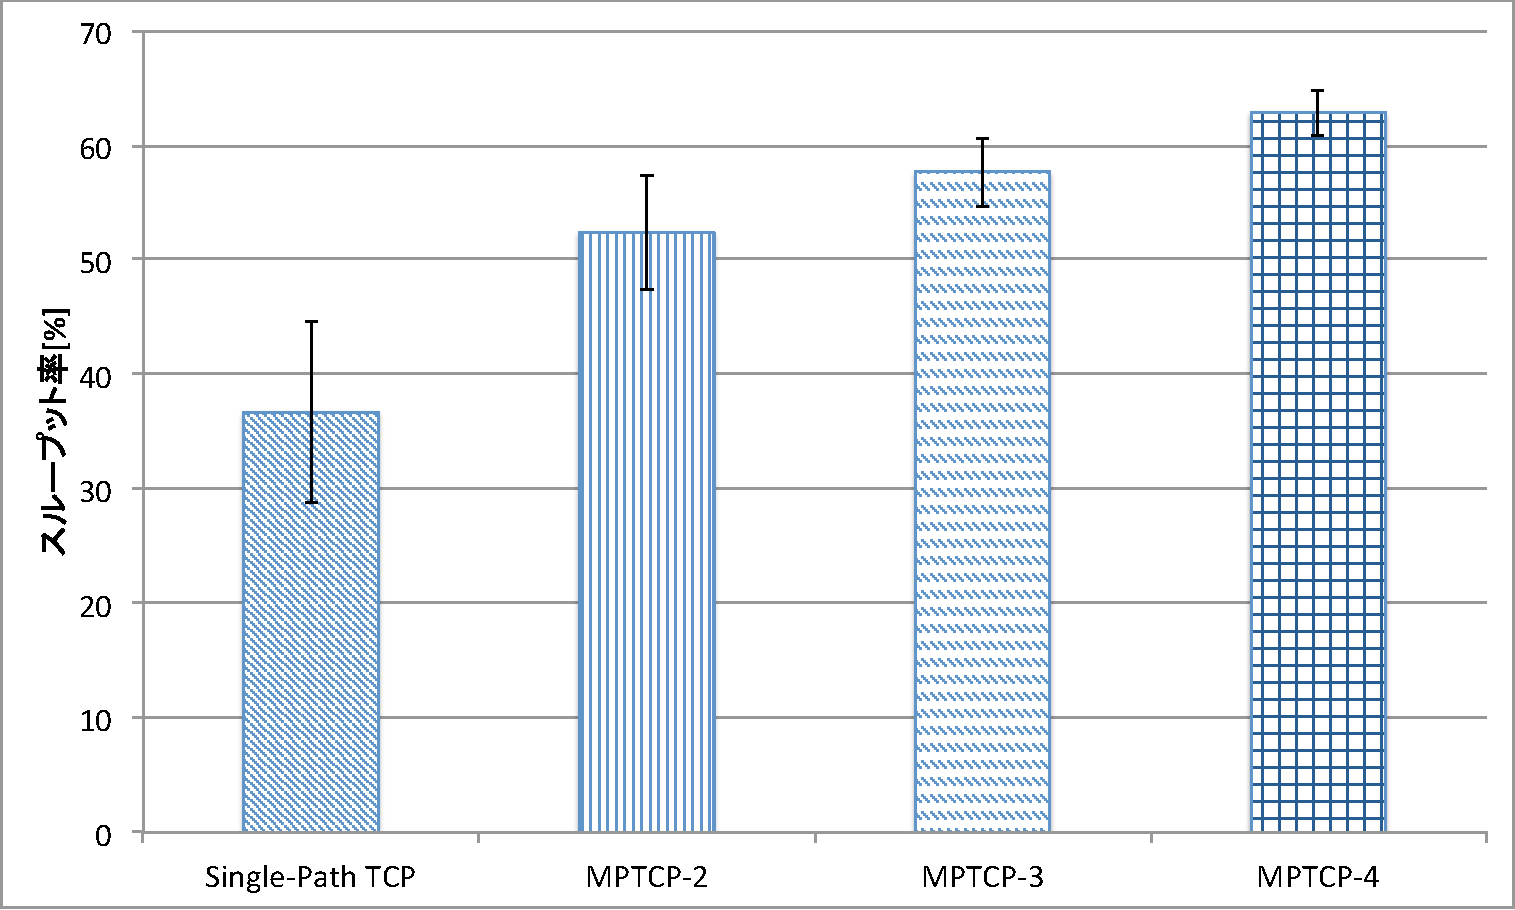
\includegraphics[autoebb, width=180pt]{./img/back.pdf}
%     \caption{Throughput of background traffic}
%     \label{fig:background}
%     \end{center}
% \end{figure}
% \hspace{1cm}

\section{あとがき}
\label{sec:conclude}
本論文では, MPTCPのフローサイズの小さいトラフィックに対しては,
従来のTCPよりもデータ転送に時間がかかるという報告~\cite{improving}を再現し, その原因を分析した.
その結果, 4つのフローパターンに分類することができ, そのうち, パケットロスが生じるフローがデータ転送時間に影響を及ぼすということを示した.
特に, MPTCPではフローサイズの大きいトラフィックが小さいトラフィックを圧迫し, パケットロスを引き起こす割合が高く,
その輻輳制御の公平性に問題が有るということを示した.
このことから, MPTCPが帯域を占有する問題を解消できれば, 従来のTCPを用いたデータセンターモデルよりも多様なトラフィックに対し性能の向上を期待される.

今後はトラフィック監視により, パケット衝突を引き起こさないロードバランスにより,
フローサイズによらずデータ転送高速化技術について検証していく予定である.

%\bibliographystyle{sieicej}
%\bibliography{myrefs}
\begin{spacing}{0.7}
\footnotesize{
\begin{thebibliography}{99}% 文献数が10未満の時 {9}
\bibitem{IBM_rep}{日本アイ・ビー・エム株式会社. IBM 第1章
大容量データのバックアップ,
\url{http://www-06.ibm.com/systems/jp/storage/column/backup/01.html}} \bibitem{amazon}{Jim Liddle. Amazon found every 100ms of latency cost them 1\%
in sales, August 2008.
\url{http://blog.gigaspaces.com/amazon-found-every-100ms-of-latency-cost}

\url{-them-1-in-sales/}}
\bibitem{presto}{Facebook. Presto: Interacting with petabytes
of data at Facebook,
\url{https://www.facebook.com/notes/facebook-engineering/presto-interacting-with-petabytes-of-data}

\url{-at-facebook/10151786197628920}}
\bibitem{mapreduce}{Dean, Jeffrey, and Sanjay
Ghemawat. "MapReduce: simplified data processing on large clusters." Communications of the ACM 51.1 (2008): 107-113.} \bibitem{dryad}{Isard, Michael, et al. "Dryad: distributed data-parallel
programs from sequential building blocks." ACM SIGOPS Operating Systems Review 41.3 (2007): 59-72.}
\bibitem{fattree}{Al-Fares, Mohammad, Alexander Loukissas, and Amin Vahdat. "A
scalable, commodity data center network architecture." ACM SIGCOMM Computer Communication Review. Vol. 38. No. 4. ACM, 2008.}
\bibitem{bcube}{Guo, Chuanxiong, et al. "BCube: a high performance,
server-centric network architecture for modular data centers." ACM SIGCOMM Computer Communication Review 39.4 (2009): 63-74.}
\bibitem{vl2}{Greenberg, Albert, et al. "VL2: a scalable and flexible data
center network." ACM SIGCOMM Computer Communication Review. Vol. 39. No. 4. ACM, 2009.}
\bibitem{dctcp}{Alizadeh, Mohammad, et al. "Data center tcp (dctcp)." ACM SIGCOMM Computer Communication Review 40.4 (2010): 63-74.}
\bibitem{improving}{Raiciu, Costin, et al. "Improving datacenter performance and
robustness with multipath TCP." ACM SIGCOMM Computer Communication Review. Vol. 41. No. 4. ACM, 2011.}
\bibitem{detail}{Zats, David, et al. "DeTail: Reducing the flow completion time
tail in datacenter networks." ACM SIGCOMM Computer Communication Review 42.4 (2012): 139-150.}
\bibitem{click}{Kohler, Eddie, et al. "The Click modular router." ACM
Transactions on Computer Systems (TOCS) 18.3 (2000): 263-297.}
\bibitem{mptcp}{Ford, Alan, et al. TCP Extensions for Multipath Operation with
Multiple Addresses: draft-ietf-mptcp-multiaddressed-03. No. Internet draft (draft-ietf-mptcp-multiaddressed-07). Roke Manor, 2011.}
\bibitem{cong}{Raiciu, C., M. Handley, and D. Wischik. "Coupled congestion
control for multipath transport protocols." draft-ietf-mptcp-congestion-01 (work in progress) (2011).}
\bibitem{ns3}{Inria「DCE - GETTING STARTED Direct Code Execution」
\url{http://www.nsnam.org/~thehajime/ns-3-dce-doc/getting-started.html}}
\bibitem{traffic}{Benson, Theophilus, Aditya Akella, and David A. Maltz.
"Network traffic characteristics of data centers in the wild." Proceedings of the 10th ACM SIGCOMM conference on Internet measurement. ACM, 2010.}
\bibitem{mptcp_linux}{ip networking lab「MultiPath TCP - Linux Kernel
implementation」\url{http://mptcp.info.ucl.ac.be/}}
\bibitem{rtt}{Vasudevan, Vijay, et al. "Safe and effective fine-grained TCP
retransmissions for datacenter communication." ACM SIGCOMM Computer Communication Review. Vol. 39. No. 4. ACM, 2009.}
\end{thebibliography}
}
\end{spacing}


\end{document}